Our system will consist of a carbon fiber frame, either 6 underwater electric thrusters or a combination of 2 thrusters and 4 ballast tanks, a pulley powered cannon for shooting tennis balls and a mechanical arm for grasping items with a camera attached to the end. 
The carbon fiber frame will need to be held together by 3d printed connecting parts. In addition, we will need at least 2 but possibly more Arduino boards to connect to the thrusters for the purpose of switching them on and off. The Arduinos will receive input from a Raspberri pi 4 that will send the signals based on a driver directing the robot. The Raspberri pi will also receive the camera feed from the front arm of the robot.


\begin{figure}[h!]
	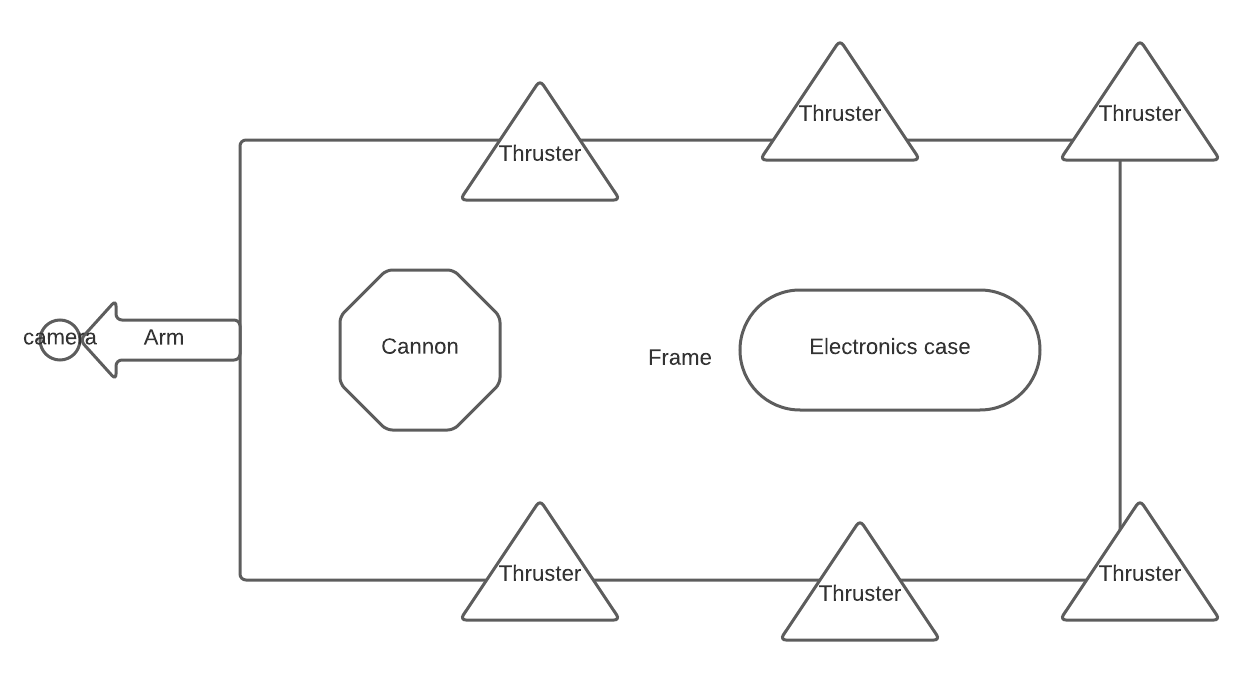
\includegraphics{images/initial_diagram.png}
\end{figure}